\chapter{Implementation\label{cha:chapter5}}

This chapter describes the implementation of the RDF instances generator and visualizer. 
Three systems were chosen as reference implementations: a VSCode version, a IntelliJ IDEA version and a Browser version. 
\section{Environment\label{sec:env}}
The following software, respectively operating systems, were used for the implementation:

\subsection{Software and development tools\label{sec:os}}

\begin{itemize}
  \item MacOS Sequoia: used during the entire development process as main Operative System.
  \item Windows 11: used to test the extension for VSCode and IntelliJ installed in a Windows environment.
  \item Visual Studio Code: used to develop the web service and the VSCode extension.
  \item IntelliJ IDEA: used for the development of the IntelliJ IDEA extension.
  \item Docker: used to create a virtual environment for the web service.
  \end{itemize}

\subsection{Programming languages, SDKs, and libraries\label{sec:proglang}}

\begin{itemize}
    \item Yeoman and VSCode Extension Generator: used to scaffold a TypeScript project ready for development.
		\item TypeScript and Node.js: used as primary programming language and package management for the VSCode extension.
		\item Kotlin and Gradle: used for the development and packaging of the IntelliJ IDEA extension.
		\item Python and pip: used for the implementation and package management of the web service.
		\item FastAPI: main Python library for the creation of a REST web service.
		\item rdflib: Python library for handling and processing RDF.
		\item sparqlwrapper: library that simplifies the use of SPARQL in Python. 
		\item vis.js: JavaScript library for creating interactive RDF graphs.
\end{itemize}

\section{Project Structure\label{sec:projectstructure}}

The implementation is separated into 3 distinguished projects as depicted in figure \ref{fig:projectstructure}.

\begin{figure}[htb]
  \centering
  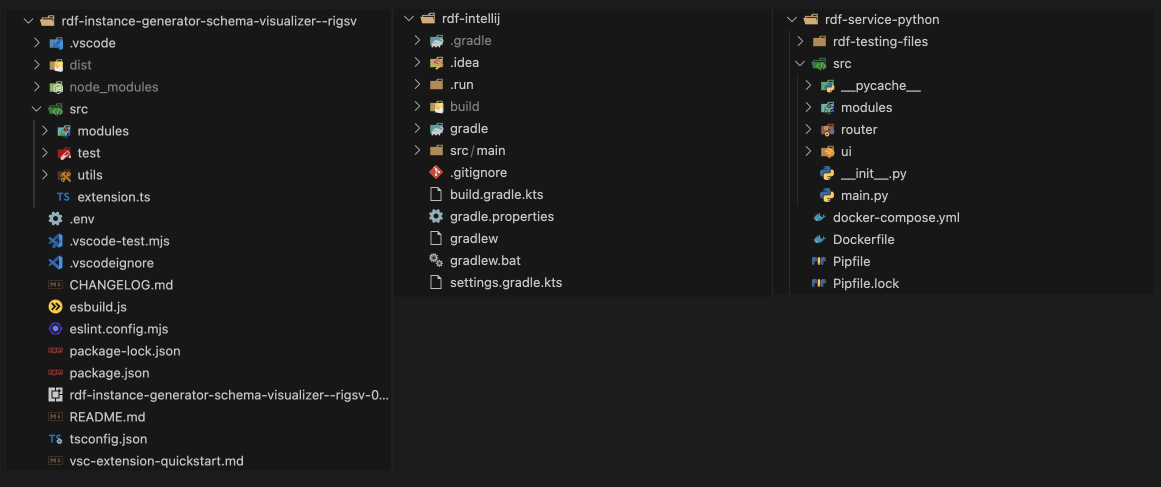
\includegraphics[width=13cm]{folder_structure.png}
  \caption{Project Structure}
  \label{fig:projectstructure}
\end{figure}

The first project is the web service (rdf-service-python), the second one is the VSCode extension (rdf-instance-generator-schema-visualizer--rigvs) and the last one is the IntelliJ plugin (rdf-IntelliJ).

\section{Implementation Web Service\label{sec:webservice}}

\begin{figure}[htb]
	\centering
	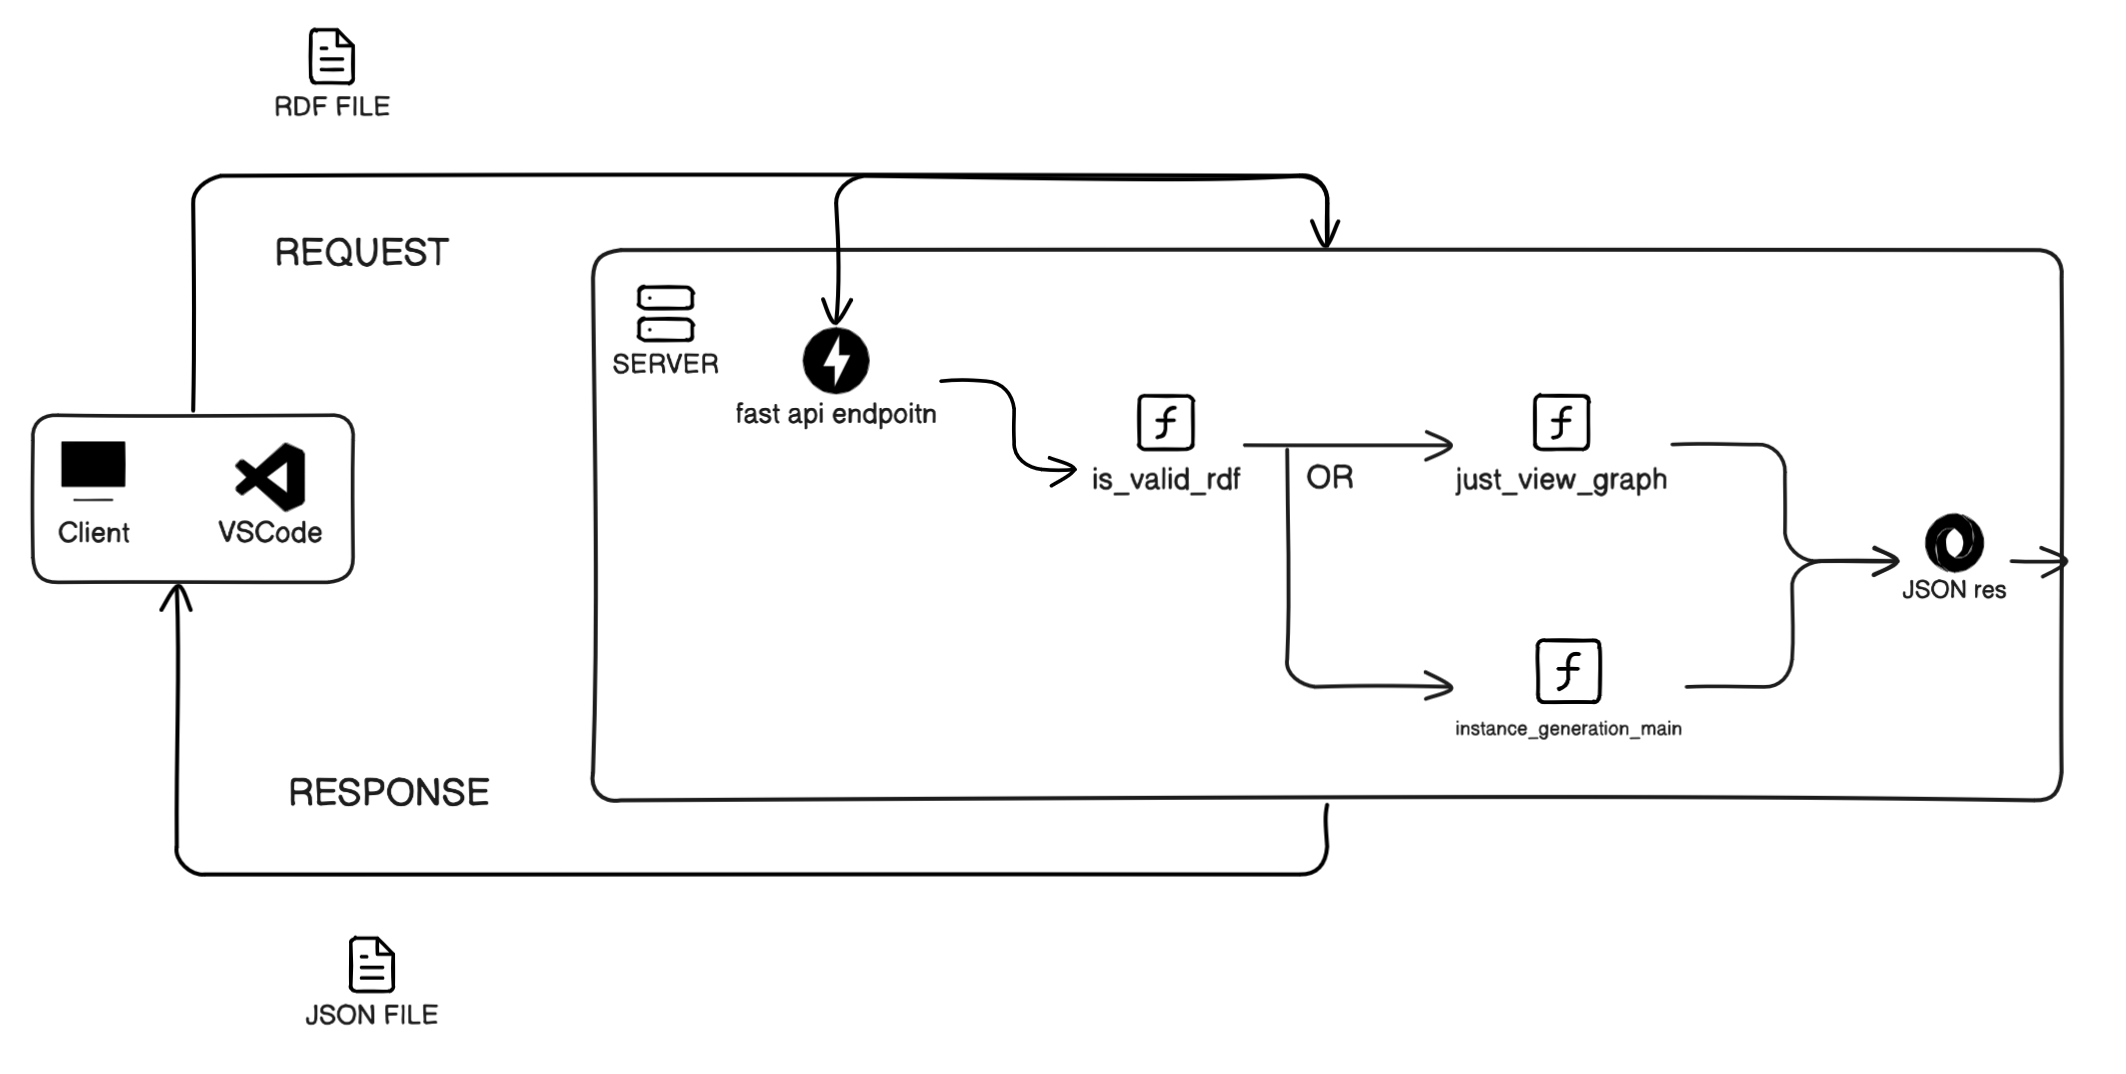
\includegraphics[width=13cm]{server_schema.png}
	\caption{Server Schema}
	\label{fig:serverschema}
  \end{figure}


\noindent
The following section describes in details the implementation of the web service with all its key components.
\\
\\
\subsection{Server} 
There are many Python libraries that allow to create a REST web service. Among them, FastAPI was the chosen one. It is a modern, fast (high-performance), web framework for building APIs with Python based on standard Python type hints \cite{fastapi}.
\\
The first step, in order to start the server, was to install FastAPI and its dependencies. After than, by simplying initializing the app object, \textbf{app = FastAPI()} and execute the \textbf{fastapi dev src/main.py} command, the server will be up and running. 
\\
\\
The next step was to create the endpoints. In src/router/router.py, the \textbf{router = APIRouter()} was initialized and three endpoints where created: to for the Browser Client and one for the extensions.
\\
\\
The first endpoint, \textbf{$router.get("/", response\_class=HTMLResponse)$}, is simply used to server the index.html file to the web Browser. This page allows the upload of RDF (POST to the next endpoint), visualize the generated graph and see the RDF file with the new generated instances.
\\
\\
The next endpoint is the \textbf{$router.post("/generate", tags=["users"])$}. This endpoint accepts incoming POST requests from the Web Browser with the incoming RDF file. It returns the required data in a JSON format.
\\
\\
The last endpoint, \textbf{$router.post("/", response\_class=JSONResponse)$}, accepts incoming POST requests from the VSCode and IntelliJ extensions. It returns data in a JSON format.
\\
\\
\subsection{RDF Validation} 
When an endpoint function receive an RDF file, the first function to be called is the \textbf{$is\_valid\_rdf(file)$}. This asynchronous function is responsible for validating the incoming RDF file. First it extracts the file extension from the incoming file. The extension name must be present in the predefined dictionary. If it's not there, an error is returned otherwise it proceed to the next step.
\\
To see if the code in the file is correct syntactically and semantically, the function uses the \textbf{rdflib} library. This function allows to parsing and serialization of RDF data, storing of RDF triples, accessing to remote SPARQL endpoints, and working with RDF graphs \cite{rdflib}.
The core of this function relies heavily on the $Graph.parse()$ method. If the file is syntactically correct and a new RDF graph is generated, then it means that the RDF is valid and the function returns true. Otherwise, it returns false.
\subsection{Graph generator}
After verifying the file is valid, the next step was to create the actual graph generation function. The $getGraph()$ uses the previously stated method for parsing the RDF file and return the graph, the file extension name and file format name to the $just\_view\_graph()$ function. 
\\
The retrieved graph is then serialized in the requested format and in json-ld.

\subsection{Instance and Graph generator}
This was the most important and complex functionality of the entire project. 
Like it has been done in the previous function, the graph, the format and the extension name are returned from the $getGraph()$.
Then a new graph is initialized and, to keep things consistent and readable, all the namespace prefixes are copied from the initial retrieved graph ($or\_graph$).
This helps make the RDF output cleaner and easier to read, since it avoids repeating long URIs and keeps the format consistent.
\\
\\
The next step is the scanning of the RDF graph. The $scan()$ function goes through the entire graph and extract classes and properties. The code then splits and creates two different functionalities: instance generation without properties search and instance generation with properties search.
\\
\\
In RDF vocabularies, classes can be either explicitly declared (e.g. $rdf:type rdfs:Class$) or implicitly referred with their usages in properties definitions (e.g. $rdfs:range schema:Car$).
In the scenario where the instance generation is executed without the properties, the code needs to generate and instance for every single class that has been found in the code, both explicitly or implicitly referred. 
\\
The $generate\_instance()$ function, take as parameters the class uri that has been extracted previously, the new graph initialized before, the number of instances that the user wants to generate for each declared class and the properties that has been defined. 
It's important to sate that the user has no control over the number of instances that come from a implicitly referred class.
\\
\\
Once the parameters are set, the function starts by checking i the class uri starts with \textbf{http://www.w3.org/2001/XMLSchema} and in case of a positive answer it skips the instance generation for that class.
\\
\\
After that, the $processed\_instances$ and $initialized\_instances$ are declared. The first, since $generate\_instance$ is a recursive function, is used for tracking which instances have already been generated to avoid duplicates. 
The second tracks which properties have been assigned to each generated instance.
\\
\\
In the next step, the function iterates N times to create multiples instances for the provided class. For each iteration, a new URI is created by using the EX prefix, the class name, and the number of the iteration (e.g. $ex:Employee\_Instance1$). If the instance has already been processed, it is simply reused from $processed\_instances$. The newly created instance is then linked to its class uri and added to the graph. 
\\
\\
If the class has any associated property, the function checks every property and handles three main cases: 
\begin{itemize}
	\item If the provided value is a URI and it is a primitive datatype, thanks to the support of a hashmap (i.e. XSD) containing the primitive types with example values, a new literal is generated and appended to the graph. If the URI is not primitive, it is treated as a reference to another class. The function calls itself recursively to generate the required number of sub-instances for the referenced class. The resulting sub-instance is then added the graph. 
	\item If the value is a XSD datatype URI as string, a default string literal (i.e., "default"^^xsd:string) is generated and the triple added to the graph.
	\item If the value is already a literal it is directly added to the graph.
	\item If the value is unsupported, an error is thrown.
\end{itemize}
Each successful initialized property, is then stored inside $initialized\_instances$.
At the end of the loop, the function adds the generated instance to the instances list and concludes with its return.
\begin{lstlisting}[caption={Instance Generation Function}, label={lst:generate_instance}]
	EX = Namespace("http://example.org/")
	
	def generate_instance(
		class_uri,
		graph,
		num_instances=1,
		property_definitions=None,
		processed_instances=None,
		initialized_instances=None,
	):
		from rdflib.namespace import XSD
	
		xsd = {
			"http://www.w3.org/2001/XMLSchema#integer": 0,
			"http://www.w3.org/2001/XMLSchema#decimal": 0.0,
			"http://www.w3.org/2001/XMLSchema#float": 0.0,
			"http://www.w3.org/2001/XMLSchema#double": 0.0,
			"http://www.w3.org/2001/XMLSchema#string": "unknown",
			# Additional types can be added as needed
		}
	
		# Skip primitive XSD types
		if str(class_uri).startswith("http://www.w3.org/2001/XMLSchema#"):
			return []
	
		instances = []
		processed_instances = processed_instances or {}
		initialized_instances = initialized_instances or {}
	
		class_name = class_uri.split("/")[-1]
	
		for i in range(num_instances):
			instance_uri = EX[f"{class_name}_Instance{i + 1}"]
	
			if instance_uri in processed_instances:
				instances.append(instance_uri)
				continue
	
			processed_instances[instance_uri] = True
			graph.add((instance_uri, RDF.type, class_uri))
	
			if property_definitions and class_uri in property_definitions:
				for prop, value in property_definitions[class_uri].items():
					if isinstance(value, URIRef):
						if str(value).startswith("http://www.w3.org/2001/XMLSchema#"):
							graph.add((instance_uri, prop,
									   Literal(xsd[str(value)], datatype=value)))
						else:
							sub_instances = generate_instance(
								value,
								graph,
								num_instances=i + 1,
								property_definitions=property_definitions,
								processed_instances=processed_instances,
								initialized_instances=initialized_instances
							)
							if sub_instances:
								value = sub_instances[i]
								graph.add((instance_uri, prop, value))
					elif str(value) in xsd:
						graph.add((instance_uri, prop,
								   Literal(xsd[str(value)], datatype=URIRef(value))))
					elif isinstance(value, Literal):
						graph.add((instance_uri, prop, value))
					else:
						raise ValueError(
							f"Unsupported value type: {type(value)} for property {prop}"
						)
	
					if instance_uri not in initialized_instances:
						initialized_instances[instance_uri] = set()
					initialized_instances[instance_uri].add(prop)
	
			instances.append(instance_uri)
	
		return instances
\end{lstlisting}

	% TODO : Continue from here with with property search
	In the scenario where the instance generation is executed with the properties means that also the side instance have properties bla bkla review this sentence

\begin{lstlisting}[caption={Main Function for RDF Instance Generation}, label={lst:instance_generation_main}]
	async def instance_generation_main(file, n=2, property_search=False):
		or_graph, format, fileFormatName = await getGraph(file)
	
		if or_graph is None:
			return None
	
		new_instances_graph = Graph()
		for prefix, namespace in or_graph.namespace_manager.namespaces():
			new_instances_graph.namespace_manager.bind(prefix, namespace)
	
		# Detect classes and their properties
		classes = scan(or_graph)
		property_definitions = {
			class_uri: details["properties"]
			for class_uri, details in classes.items()
		}
	
		if property_search == True:
			undeclared_classes_props = find_properties(classes, 1)
			new_property_definitions = update_props(property_definitions, undeclared_classes_props)
	
			for class_uri in classes:
				generate_instance(
					class_uri,
					new_instances_graph,
					num_instances=n,
					property_definitions=new_property_definitions
				)
		else:
			for class_uri in classes:
				generate_instance(
					class_uri,
					new_instances_graph,
					num_instances=n,
					property_definitions=property_definitions
				)
	
		rdf_data = save_to_new_response(or_graph, new_instances_graph, fileFormatName)
		json_dl = rdf_format_json(rdf_data, fileFormatName)
	
		return {
			"data": rdf_data,
			"fileName": f"new_rdf{format}",
			"json_dl": json_dl
		}
	\end{lstlisting}

